%!TEX root = ../Fast_Contour_Tracing_Algorithm.tex
% -*- root: ../Fast_Contour_Tracing_Algorithm.tex -*-

\section{Proposed Contour-tracing Algorithm}

% In this section, we propose a novel pixel following algorithm that traces contour pixels by considering their local patterns. Therefore, it can classify the contour pixel into contour types such as inner corner, outer corner, inner-outer corner, and straight line; further, it can easily determine the next contour pixel. Moreover, it can determine and save representative points of an image, like the RD code method, by using pixel following but not using run-data-based following. In addition, the data can be restored to the original contour pixels without the RD code data.

In this section, we propose a novel pixel-following algorithm that traces contour pixels by considering their local patterns. Therefore, it can classify the contour pixel as inner corner, outer corner, inner-outer corner, and straight-line contour types. Further, it can easily determine the next contour pixel. Moreover, it can determine and save representative points of an image, such as the RD code method, by using pixel following but not using run-data-based following. In addition, the data can be restored to the original contour pixels without the RD code data.

\subsection{Contour Following}

\subsubsection{Assumptions for Start-up and Stopping Criteria}

% The proposed algorithm runs under two assumptions for start. One is the general condition for pixel following: the rear pixel of the tracer on the start pixel is white. The other is that there is no left-rear inner-outer corner for the tracer at the start position, i.e., if the rear and the left pixels are white and the rear-left pixel is black, the start pixel has to be changed. These are the same starting conditions as those for the MSBF and ISBF. Moreover, the stop criteria of the proposed algorithm is Jacob's stopping criterion and the tracer is always on a contour pixel.

The proposed algorithm runs under two assumptions for starting. One is the general condition for pixel following, where the rear pixel of the tracer on the start pixel is white. The other is that there is no left-rear inner-outer corner for the tracer at the start position, i.e., if the rear and the left pixels are white and the rear-left pixel is black, the start pixel has to be changed. These are the same starting conditions as those used for the MSBF and ISBF. Moreover, the stop criteria of the proposed algorithm is Jacob's stopping criterion, and the tracer is always on a contour pixel. 

% Image 9
\begin{figure}[htbp]
	\centering
	\subfloat[]{ 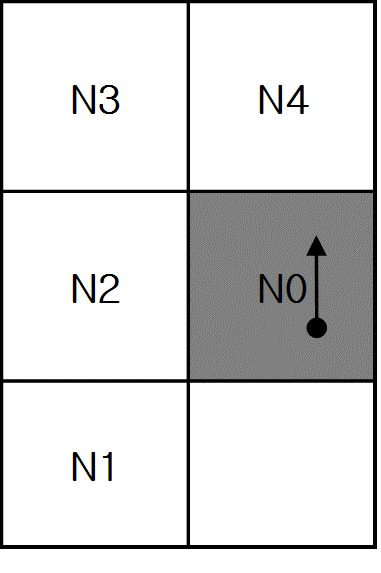
\includegraphics[width=0.25\textwidth]{4.Proposed/fig9-a.png} \label{fig:img9-a} }
	\subfloat[]{ 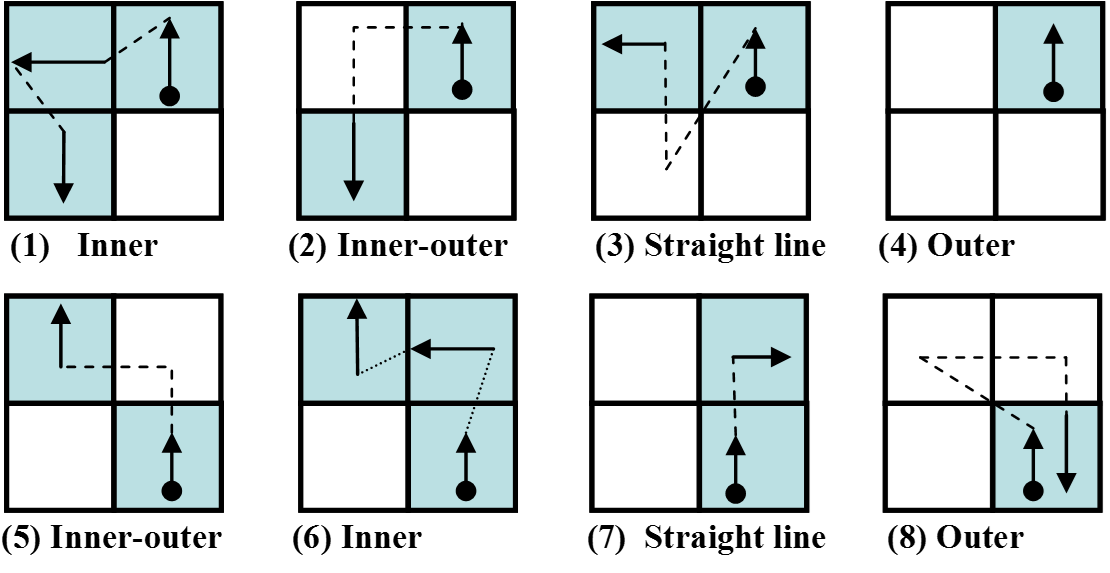
\includegraphics[width=0.73\textwidth]{4.Proposed/fig9-b.png} \label{fig:img9-b} }

	\caption{Contour Tracing Cases for Proposed Contour-following Algorithm. \protect\subref{fig:img9-a} Adjacent pixels \protect\subref{fig:img9-b} Contour cases}
	\label{fig:image9}
\end{figure}


\subsubsection{Procedures}

% The proposed algorithm has two stages. First, the tracer follows the contour pixel on the basis of the intensities of the left-rear and left pixels. After that, the tracer follows the contour pixels on the basis of the intensities of the front and front-left pixels. Figure \ref{fig:image9} shows the contour tracing cases of the proposed contour following algorithm. In the figure, the tracer is first on $N0$ queries states of $N1$ and $N2$, as shown in figure \ref{fig:image9} (a), and then the states determine the corresponding  path to trace among cases (1)-(4), as shown in figure \ref{fig:image9} (b). After stage 1, the moved tracer queries states N3 and N4 and then it traces contour pixels along the corresponding path using the states among cases (5)-(8). 

The proposed algorithm has two stages. First, the tracer follows the contour pixel based on the intensities of the left-rear and left pixels. After that, the tracer follows the contour pixels according to the intensities of the front and front-left pixels. Figure \ref{fig:image9} shows the contour tracing cases for the proposed contour-following algorithm. In the figure, the tracer is first on $N0$ queries states of $N1$ and $N2$, as shown in Figure \ref{fig:img9-a}, and then the states determine the corresponding path to be traced from among cases (1)-(4), as shown in Figure \ref{fig:img9-b}. After stage 1, the moved tracer queries states $N3$ and $N4$, and it then traces contour pixels along the corresponding path using the states from among cases (5)-(8). 

% Hence, by using the proposed algorithm, the inner corners are traced as case (1) or case (6), the inner-outer corners are traced as case (2) or case (5), the outer corners are determined as case (4) or case (8), and the straight-line pixels are determined as the other cases. Therefore, all the cases are easily classified by using the algorithm. 

Hence, by using the proposed algorithm, the inner corners traced are considered as case (1) or case (6), the inner-outer corners are considered as case (2) or case (5), the outer corners are considered as case (4) or case (8), and the straight-line pixels are considered as the other cases. Therefore, all the cases are easily classified using the algorithm. 




\subsubsection{States}

% Image 10
\begin{figure}[htbp]
	\centering
	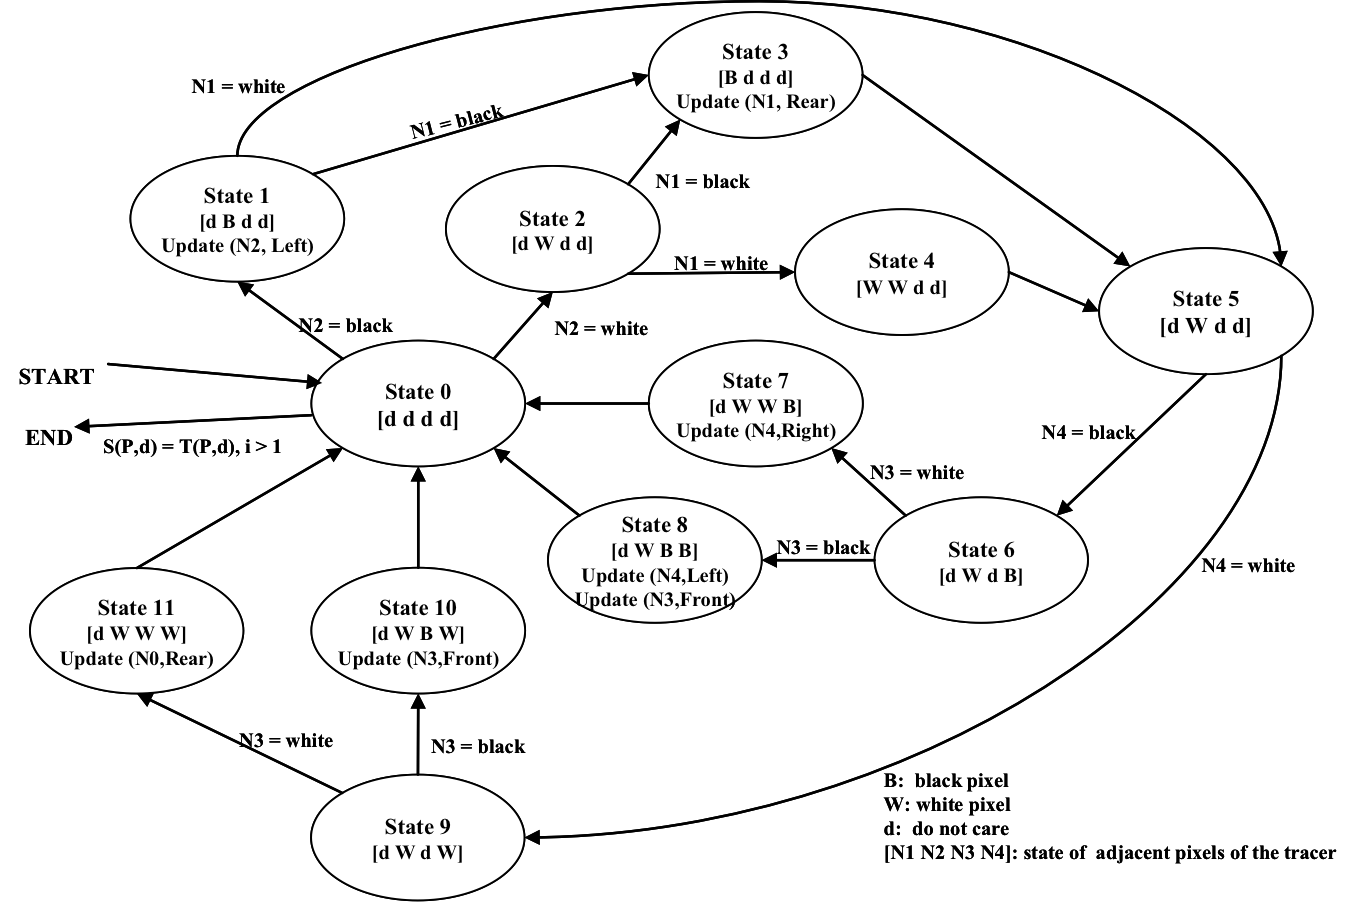
\includegraphics[width=1.0\textwidth]{4.Proposed/state.png}
	\caption{State Transition of Automation for Proposed Algorithm.}
	\label{fig:image10}
\end{figure}

% Figure \ref{fig:image10} describes the state transition for the automation of the proposed algorithm. In the figure, the start and termination occur at State 0; the first stage runs using States 1-4 and then it transits to State 5. The second stage continues from State 5 using States 6-11 and then it transits to State 0. For example, case (1) in figure \ref{fig:image9} can be executed by the transit sequence State 1, State 3, and State 5. 

Figure \ref{fig:image10} describes the state transition for the automation of the proposed algorithm. In the figure, the start and termination occur at State 0. The first stage runs using States 1-4, and it then transits to State 5. The second stage continues from State 5 using States 6-11, and it then transits to State 0. For example, case (1) in Figure \ref{fig:img9-b} can be executed using the transit sequence State 1, State 3, and State 5.

% In figure \ref{fig:image10}, $[N1 N2 N3 N4]$ represents the intensity vector of the tracer's four adjacent pixels shown in figure \ref{fig:image9} (a). In the vector, $d$ implies ``do not care''; $B$, a contour pixel (black); and $W$, the background pixel (white). Moreover, Update $(P,d)$ refers to the movement operation where $P$ is the new contour pixel location and $d$ is the new directional information for the tracer. In State 1 and State 3, the updates occur based on the tracer of State 0, and other updates are based on the tracer information in State 5.

In Figure \ref{fig:image10}, $[N1\ N2\ N3\ N4]$ represents the intensity vector of the tracer's four adjacent pixels shown in Figure \ref{fig:img9-a}. In the vector, $d$ implies ``do not care''; $B$ represents a contour pixel (black), and $W$ represents the background pixel (white). Moreover, Update $(P,d)$ refers to the movement operation where $P$ is the new contour-pixel location and $d$ is the new directional information for the tracer. In States 1 and 3, the updates occur based on the tracer of State 0, and other updates are based on the tracer information in State 5.

\subsubsection{Characteristics of Proposed Algorithm}

% We designed the proposed algorithm based on two stages with two major goals. First, the check operation for stopping occurs only at State 0; therefore, the number of checking operations on black pixels are reduced. In other words, the proposed algorithm examines that the check operation occurs when only the tracer has a white rear pixel. This is more efficient as compared to the check operation occuring for every contour pixel because its start condition and stop criterion also satisfy that the rear pixel of the tracer on the start pixel is white. Therefore, the transition of stage 2 to States 6 to 11 for processing cases (5) to (8) is designed such that it can be returned to State 0 only if the tracer has a white rear pixel, and it reduces any unnecessary operations for checking to stop. Besides, the tracers of cases (2) and (4) have a white rear pixel after movement but their end conditions are not considered. In case (2), at the start the tracer avoids the inner-outer corner pixels as the start and end pixel. Moreover, in case (4), the tracer has no update; therefore, it is unnecessary to perform check operation twice. 

We designed the proposed algorithm based on two stages with two major goals. First, the check operation for stopping occurs only at State 0; therefore, the number of checking operations on black pixels is reduced. In other words, the proposed algorithm verifies that the check operation occurs when only the tracer has a white rear pixel. This is more efficient when compared to the check operation that occurs for every contour pixel because its start condition and stop criterion also satisfy the condition that the rear pixel of the tracer on the start pixel should be white. Therefore, the transition of stage 2 to States 6-11 for processing cases (5) to (8) is designed such that it can be returned to State 0 only if the tracer has a white rear pixel, and it reduces any unnecessary operations that are required to stop the checking. Besides, the tracers of cases (2) and (4) have a white rear pixel after the movement, but their end conditions are not considered. In case (2), at the start, the tracer avoids the inner-outer corner pixels as the start and end pixel. Moreover, in case (4), the tracer has no update; therefore, it is unnecessary to perform the check operation twice. 

% Second, the proposed algorithm reduces some of the redundant operations used for detecting white pixels. The conventional algorithms do not consider white pixels in the previous path; therefore, they sometimes redetect white pixels on the previous tracing during the current tracing. For example, in figure 8, the white pixel at (4, 2) is detected twice while determining contour pixels such as (4, 3) and (5, 3). Moreover, RSA detects (4, 2) three time while determining (4, 3), (5, 3), and (6, 3). On the contrary, the proposed algorithm has two stages and its second stage avoids the previous path. \textcolor{red}{Figure 11} shows the contour tracing results for the proposed algorithm and it detects (4, 2) once for contour tracing. Moreover, the figure shows that the proposed algorithm has fewer operations on the white pixels as compared to conventional pixel following methods, as shown in figure \ref{fig:image8}, and traces all the types of contours. 

Second, the proposed algorithm eliminates some of the redundant operations that are used to detect white pixels. The conventional algorithms do not consider white pixels in the previous path; therefore, they sometimes redetect white pixels on the previous tracing during the current tracing. For example, in Figure \ref{fig:image8}, the white pixel at $(4, 2)$ is detected twice while determining contour pixels such as $(4, 3)$ and $(5, 3)$. Moreover, RSA detects $(4, 2)$ three times while determining $(4, 3)$, $(5, 3)$, and $(6, 3)$. On the contrary, the proposed algorithm has two stages, and its second stage avoids the previous path. Figure \ref{fig:image11} shows the contour-tracing results obtained for the proposed algorithm, and it detects $(4, 2)$ once for contour tracing. Moreover, the figure shows that the proposed algorithm has fewer operations on the white pixels when compared to conventional pixel-following methods, as shown in Figure \ref{fig:image8}, and it traces all types of contours. 

% Image 11
\begin{figure}[htbp]
	\centering
	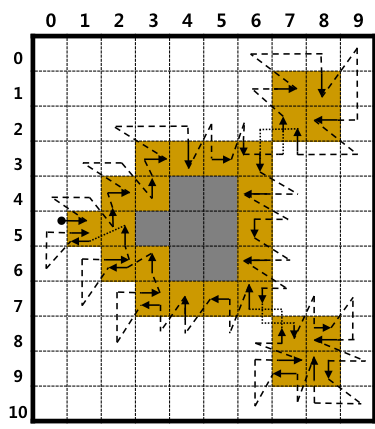
\includegraphics[width=0.4\textwidth]{4.Proposed/fig11.png}
	\caption{Result of contour tracing using proposed algorithm}
	\label{fig:image11}
\end{figure}

% The pseudo-code of the proposed algorithm is as below: 

The pseudocode of the proposed algorithm is given below: 

\begin{algorithm}
	\caption{Procedure of Proposed Tracer}
	\label{alg:proposed}
	\begin{algorithmic}[1]
	\Procedure{Proposed\_Tracer}{}
	\State $\textit{T(P,d)} \gets \textit{S(P,d)}$, where $P$ is on black, $P_{Rear}$ is on white and $i \gets 1$
	\LineComment{Whenever $T(P,d)$ is updated, $i$ increases $1$ and $T(p',d')$ is saved automatically}
	\Do
	\LineComment{Stage 1}
	\If {$\textit{P}_{Left-Rear}$ = black}
		\If {$\textit{P}_{Left}$ = black}
			\LineComment{Case 1}
			\State $\textit{T(P,d)} \gets \textit{T(P}_{Left},\textit{d}_{Left} )  $ and $\textit{Code(i)} \gets ``Inner''$
			\State $\textit{T(P,d)} \gets \textit{T(P}_{Left}, \textit{d}_{Left})$
		\Else
			\LineComment{Case 2}
			\State $\textit{Code(i)} \gets ``Inner-outer''$
			\State $\textit{T(P,d)} \gets \textit{T(P}_{Left-Rear},\textit{d}_{Rear} )  $ and $\textit{Code(i)} \gets ``Inner-outer''$
		\EndIf
	\Else
		\If {$\textit{P}_{Left}$ = black}
			\LineComment{Case 3}
			\State $\textit{T(P,d)} \gets \textit{T(P}_{Left},\textit{d}_{Left} )  $ and $\textit{Code(i)} \gets ``Straight''$
		\Else
			\LineComment{Case 4}
			\State $\textit{Code(i)} \gets ``Outer''$
		\EndIf
	\EndIf


	\LineComment{Stage 2}
	\If {$\textit{P}_{Front-Left}$ = black}
		\If {$\textit{P}_{Front}$ = black}
			\LineComment{Case 6}
			\State $\textit{T(P,d)} \gets \textit{T(P}_{Front},\textit{d}_{Left} )  $ and $\textit{Code(i)} \gets ``Inner''$
			\State $\textit{T(P,d)} \gets \textit{T(P}_{Front}, \textit{d}_{Right})$
		\Else
			\LineComment{Case 5}
			\State $\textit{Code(i)} \gets ``Inner-outer''$
			\State $\textit{T(P,d)} \gets \textit{T(P}_{Front-Left},\textit{d} )  $ and $\textit{Code(i)} \gets ``Inner-outer''$
		\EndIf
	\ElsIf {$\textit{P}_{Front}$ = black}
		\LineComment{Case 7}
		\State $\textit{T(P,d)} \gets \textit{T(P}_{Front},\textit{d}_{Right} )  $
	\Else
		\LineComment{Case 8}
		\State $\textit{T(P,d)} \gets \textit{T(P},\textit{d}_{Rear} )  $ and $i \gets i-1$ and $\textit{Code(i)} \gets ``Outer''$
	\EndIf


	\doWhile {$ \textit{T(P,d)}  \neq \textit{S(P,d)}$}
	\EndProcedure
	\end{algorithmic}
\end{algorithm}

% Table \ref{table:table2} describes the tracing results obtained by using the proposed algorithm up to the stage the tracer enters the 11th pixel. The code represents the contour pixel type and it is classified automatically during tracing. 

Table \ref{table:table2} describes the tracing results that were obtained by using the proposed algorithm up to the stage at which the tracer enters the 11th pixel. The code represents the contour pixel type, and it is classified automatically during tracing. 

\begin{table}[h]
	\centering
	\begin{tabularx}{0.7\textwidth}{YYYY}
		\toprule
		\multirow{2}{*}{$Sequence(i)$} &  \multicolumn{2}{c}{P}  & \multirow{2}{*}{$Code(i)$} \\
		% \cline{2-3}
		             &$x$       & $y$ & \\
		\midrule
		1 & 1 & 5 & Outer \\
		2 & 2 & 5 & Inner \\
		3 & 2 & 4 & Outer \\
		4 & 3 & 4 & Inner \\
		5 & 3 & 3 & Outer \\
		6 & 4 & 3 & Straight \\
		7 & 5 & 3 & Straight \\
		8 & 6 & 3 & Inner-outer \\
		9 & 7 & 2 & Inner-outer \\
		10 & 7 & 1 & Outer \\
		11 & 8 & 1 & \\

		\bottomrule
	\end{tabularx}
	\caption{Result Table of the Proposed Contour Tracing}
	\label{table:table2}
\end{table}

% In the table, $Code (i)$ represents only one code, the contour pixel type, per contour pixel but it can have several codes, for example, there is an outer corner pixel and an inner-outer corner pixel. 

In the table, $Code (i)$ represents only one code, the contour pixel type per contour pixel, but it can have several codes. For example, there is an outer-corner pixel and an inner-outer corner pixel. 


%%%%%%%%%%%%%%%%%
 \subsection{Data Compression and Restoration}

 % The proposed algorithm saves representation points and the inner-outer corner points in the form of compressed data in order to reduce the data size. The representation points are feature points that are used for storing and restoring contour pixels, while the inner-outer corner points are used for accurately restoring the inner-outer corner pixels. 

 The proposed algorithm saves representation points and the inner-outer corner points in the form of compressed data in order to reduce the data size. The representation points are feature points that are used for storing and restoring contour pixels, while the inner-outer corner points are used for accurately restoring the inner-outer corner pixels. 

 \subsubsection{Data Structure}
 % The representative points and inner-outer corner points are represented as vertices of contour pixels. Figure \textcolor{red}{12 (a)} shows the point types of the proposed algorithm. The representative point is of seven types, namely, two outer corners, two inner corners, and one inner-outer corner. Moreover, the inner-outer corner point has two types. Figure \textcolor{red}{12 (b)} illustrates all cases of contour tracing for the proposed algorithm and their corresponding representative points and inner-outer corner points. 

The representative points and inner-outer corner points are represented as vertices of contour pixels. Figure \ref{fig:img12-a} shows the point types of the proposed algorithm. There are seven types of representative point. They are two outer corners, two inner corners, and one inner-outer corner. In addition, there are two types of inner-outer corner point. Figure \ref{fig:img12-b} illustrates all cases of contour tracing for the proposed algorithm and their corresponding representative points and inner-outer corner points. 

 % These points are saved as a sequence during contour tracing. If an $i$-th representative point $R_i$ is equivalent to $(r_{i,x}, r_{i,y})$, then the set of representative points $R$ is given by $\{R_0, R_1, R_2, … , R_{n-1}\}$ and $R_0 = R_n$ because the starting and ending points are the same. Similarly, if $C_j$ is the $j$-th inner-outer corner point, it can be represented using its coordinate and its type. The type of the point $C_{j,T}$ is assigned to be NW-SE or NE-SW, as shown in figures \textcolor{red}{12 (a)}. Table \ref{table:data_structure} shows the data structure for data compression and restoration of the contour pixels by using the proposed algorithm. 

 These points are saved as a sequence during contour tracing. If the $i$-th representative point $R_i$ is equivalent to $(r_{i,x}, r_{i,y})$, then the set of representative points $R$ is given by $\{R_0, R_1, R_2, \cdots  , R_{n-1}\}$ and $R_0 = R_n$ because the starting and ending points are the same. Similarly, if $C_j$ is the $j$-th inner-outer corner point, it can be represented using its coordinate and its type. The type of point $C_{j,T}$ is assigned to be $NW-SE$ or $NE-SW$, as shown in Figure \ref{fig:img12-a}. Table \ref{table:data_structure} shows the data structure for data compression and the restoration of the contour pixels using the proposed algorithm. 

 %%% Image 12
\begin{figure}[htbp]
	\centering
	\subfloat[]{ 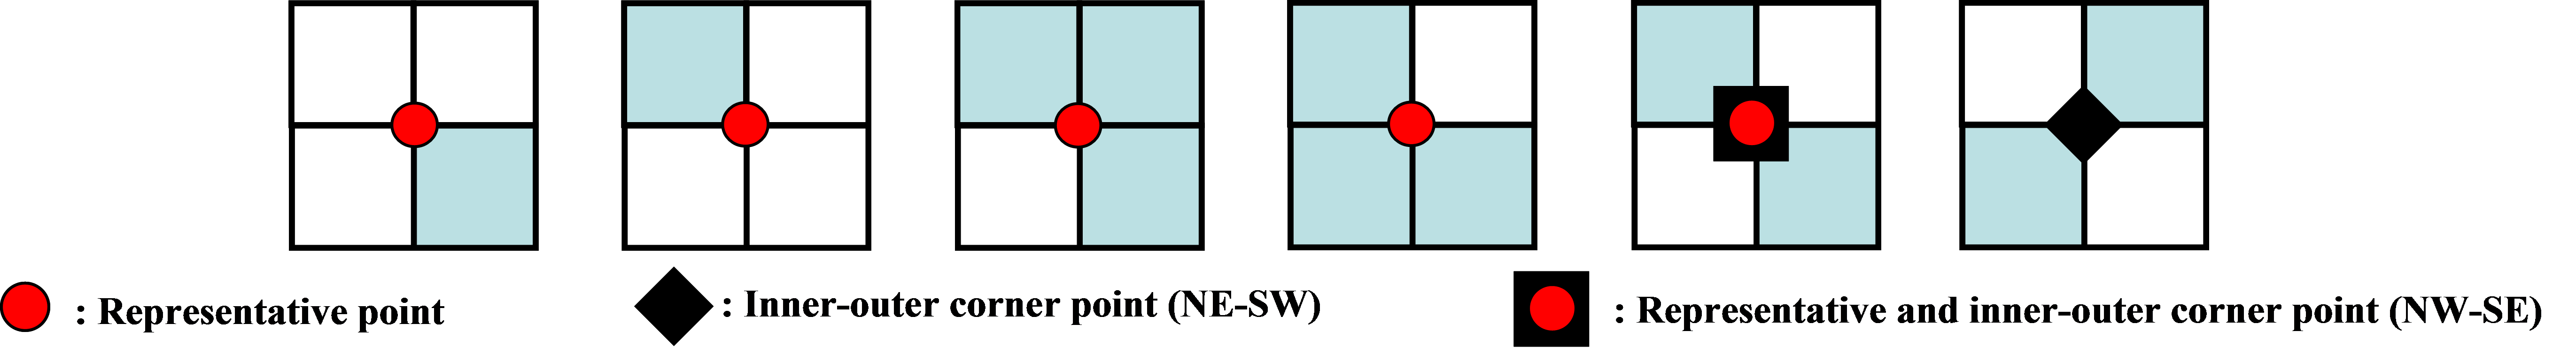
\includegraphics[width=1.0\textwidth]{4.Proposed/fig12-a.png} \label{fig:img12-a} } \\
	\subfloat[]{ 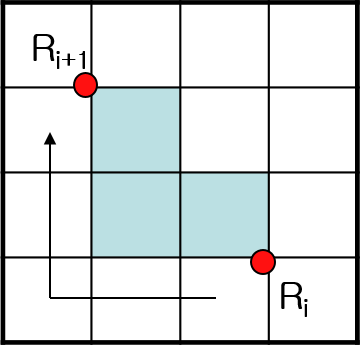
\includegraphics[width=1.0\textwidth]{4.Proposed/fig12-b.png} \label{fig:img12-b} }
	\caption{Contour Pixel Reconstruction. \protect\subref{fig:img12-a} Representative points and inner-outer corner points \protect\subref{fig:img12-b} Cases of the proposed algorithm }
	\label{fig:image12}
\end{figure}


 \begin{table}[h]
	\centering
	\begin{tabularx}{0.7\textwidth}{YYYYY}
		\toprule
		\multicolumn{2}{c}{Representative Points($R_i$)} & 
		\multicolumn{3}{c}{Inner-outer Corner($C_i$)} \\
		% \hline
		$x$ & $y$ & $x$ & $y$ & Type \\
		\midrule

		$r_{1,x}$ & $r_{1,y}$ & $C_{1,x}$ & $C_{1,y}$ & $C_{1,T}$ \\
		$r_{2,x}$ & $r_{2,y}$ & $C_{2,x}$ & $C_{2,y}$ & $C_{2,T}$ \\
		... & ... & ... & ... & ...\\
		\bottomrule
	\end{tabularx}
	\caption{Data Structure of Proposed Contour Tracer.}
	\label{table:data_structure}
\end{table}

\subsubsection{Contour Pixel Restoration}

% For restoration, we proposed a restoration algorithm comprising two stages, namely, contour restoration and inner-outer corner restoration.

For the restoration, we proposed a restoration algorithm comprising two stages, namely, contour restoration and inner-outer corner restoration.


% \subsubsection{Contour Restoration with Representation Points}
\paragraph{Contour Restoration with Representation Points}

% The sequence of representative points is important information for reconstructing the contour pixels because it represents the contour tracing sequence. Hence, by using the sequence of representative points and the relative location between adjacent representative points in the representative point table, the contour can be restored easily. If there are two sequential representative points $R_i$ and $R_{i+1}$, $\Lambda(R_i, R_{i+1})$ as the relative position classifier from $R_i$ to $R_{i+1}$ can be described as 

The sequence of representative points is important for the reconstruction of the contour pixels because it represents the contour-tracing sequence. Hence, by using the sequence of representative points and the relative location between adjacent representative points in the representative point table, the contour can be restored easily. If there are two sequential representative points $R_i$ and $R_{i+1}$, $\Lambda(R_i, R_{i+1})$, which is the relative position classifier from $R_i$ to $R_{i+1}$, can be described as 

\begin{equation}
	\Lambda(R_i, R_{i+1}) = \begin{cases}
	NE\: \text{where\:} r_{i,x} < r_{i+1,x}\: \text{and\:} r_{i,y} > r_{i+1,y} \\ 
	SE\: \text{where\:} r_{i,x} < r_{i+1,x}\: \text{and\:} r_{i,y} < r_{i+1,y} \\ 
	NW\: \text{where\:} r_{i,x} > r_{i+1,x}\: \text{and\:} r_{i,y} > r_{i+1,y} \\ 
	SW\: \text{where\:} r_{i,x} > r_{i+1,x}\: \text{and\:} r_{i,y} < r_{i+1,y}
	\end{cases}
	\label{eq:lambda}
\end{equation}

% Figure \textcolor{red}{13} shows the contour pixel reconstruction methods using the relative positions from $R_i$ to $R_{i+1}$. In the case of SE or NW, the contour pixels are filled in a clockwise manner and in the other cases, these pixels are filled in a counterclockwise manner.
Figure \ref{fig:image13} shows the contour-pixel reconstruction methods using the relative positions from $R_i$ to $R_{i+1}$. In the case of $SE$ or $NW$, the contour pixels are filled in a clockwise manner, while in the other cases, these pixels are filled in a counterclockwise manner.

%%% Image 12
\begin{figure}[htbp]
	\centering
	\subfloat[]{ 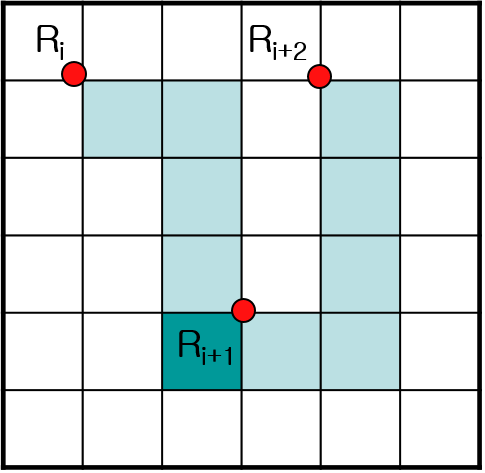
\includegraphics[width=0.24\textwidth]{4.Proposed/fig13-a.png} \label{fig:img13-a} }
	\subfloat[]{ 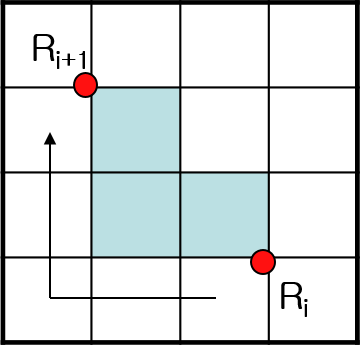
\includegraphics[width=0.24\textwidth]{4.Proposed/fig13-b.png} \label{fig:img13-b} }
	\subfloat[]{ 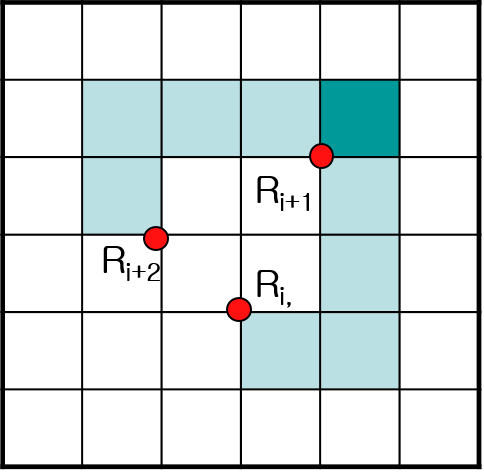
\includegraphics[width=0.24\textwidth]{4.Proposed/fig13-c.png} \label{fig:img13-c} } 
	\subfloat[]{ 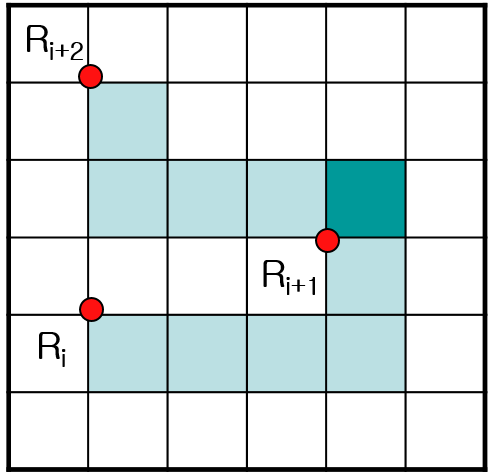
\includegraphics[width=0.24\textwidth]{4.Proposed/fig13-d.png} \label{fig:img13-d} }
	\caption{Contour Pixel Reconstruction. \protect\subref{fig:img13-a} SE \protect\subref{fig:img13-b} NW \protect\subref{fig:img13-c} SW \protect\subref{fig:img13-d} NE}
	\label{fig:image13}
\end{figure}

% The methods in figure \JHMEMO{13} are the basic methods for restoring the contour, but they have a problem in reconstructing the inner corner pixel using three or more representative points. Table \ref{table:ex_innerCornerMissing} and figure \JHMEMO{14} show cases of missing inner corner pixels using sequential representative points $R_i$, $R_{i+1}$, and $R_{i+2}$.

The methods in Figure \ref{fig:image13} are the basic methods employed to restore the contour, but they are problematic when used to reconstruct the inner-corner pixel using three or more representative points. Table \ref{table:ex_innerCornerMissing} and Figure \ref{fig:image14} show cases of the missing inner-corner pixels using sequential representative points $R_i$, $R_{i+1}$, and $R_{i+2}$.

%%% Image 13
\begin{figure}[htbp]
	\centering
	\subfloat[]{ 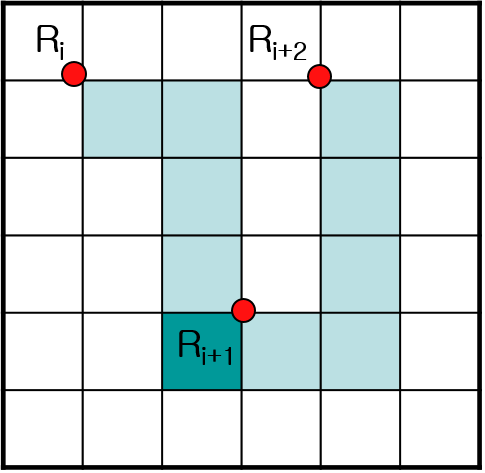
\includegraphics[width=0.24\textwidth]{4.Proposed/fig14-a.png} \label{fig:img14-a} }
	\subfloat[]{ 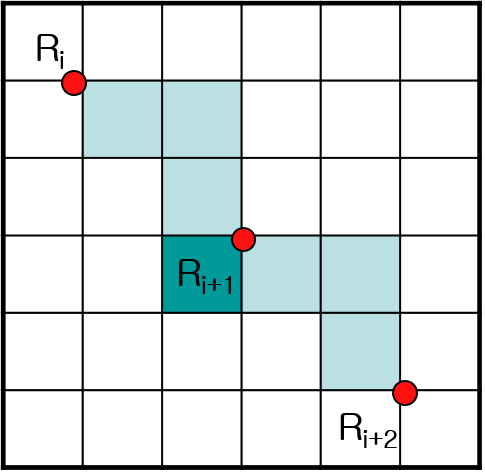
\includegraphics[width=0.24\textwidth]{4.Proposed/fig14-b.png} \label{fig:img14-b} }
	\subfloat[]{ 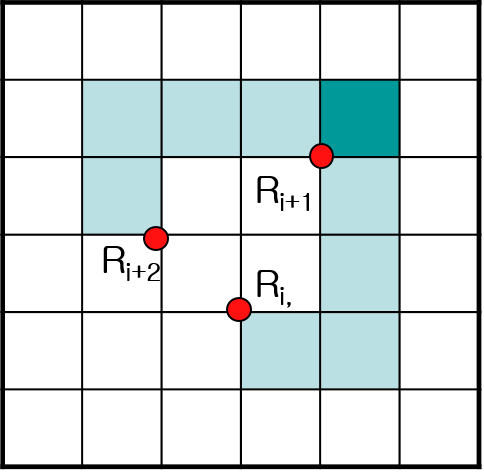
\includegraphics[width=0.24\textwidth]{4.Proposed/fig14-c.png} \label{fig:img14-c} } 
	\subfloat[]{ 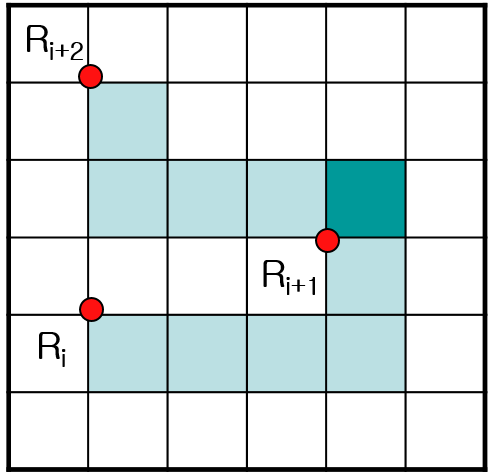
\includegraphics[width=0.24\textwidth]{4.Proposed/fig14-d.png} \label{fig:img14-d} } //
	\subfloat[]{ 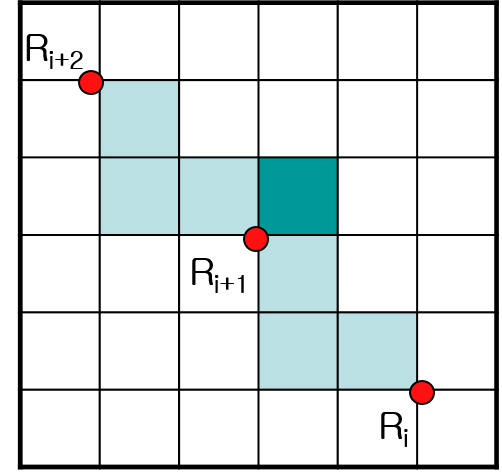
\includegraphics[width=0.24\textwidth]{4.Proposed/fig14-e.png} \label{fig:img14-e} }
	\subfloat[]{ 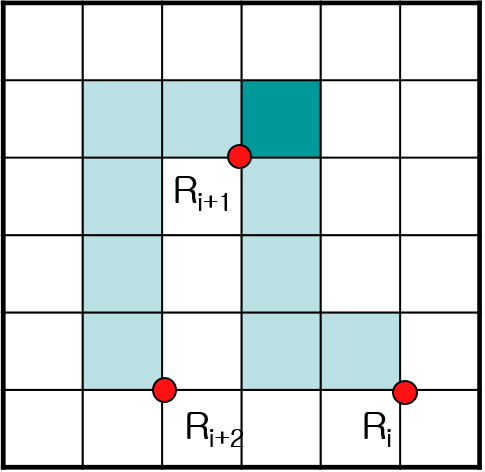
\includegraphics[width=0.24\textwidth]{4.Proposed/fig14-f.png} \label{fig:img14-f} }
	\subfloat[]{ 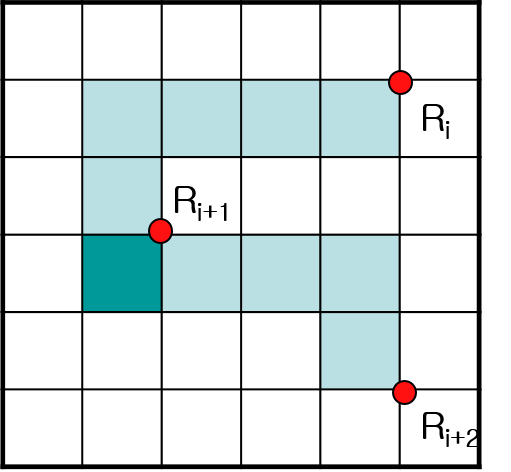
\includegraphics[width=0.24\textwidth]{4.Proposed/fig14-g.png} \label{fig:img14-g} }
	\subfloat[]{ 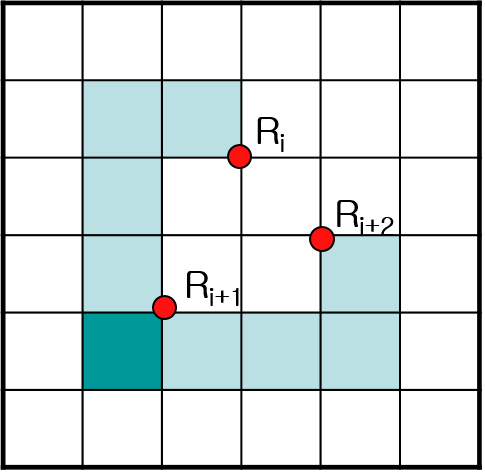
\includegraphics[width=0.24\textwidth]{4.Proposed/fig14-h.png} \label{fig:img14-h} }
	 
	\caption{Restoration Cases for Different Sequences of Representation Points. \protect\subref{fig:img14-a} - \protect\subref{fig:img14-h} Case 1 - 8}
	\label{fig:image14}
\end{figure}

 \begin{table}[h]
	\centering
	\begin{tabularx}{0.7\textwidth}{Y|Y|Y}
		\hline
		Case & $(R_i, R_{i+1})$ & $(R_{i+1}, R_{i+2})$\\
		\hline
		1 & SE & NE \\
		2 & SE & SE \\
		3 & NE & SW \\
		4 & NE & NW \\
		5 & NW & NW \\
		6 & NW & SW \\
		7 & SW & SE \\
		8 & SW & NE \\
		\hline
	\end{tabularx}
	\caption{Examples of Inner Corner Missing}
	\label{table:ex_innerCornerMissing}
\end{table}

% As shown in the figure, the three representative points cannot restore the inner corner pixel $P_m$. Therefore, if the three sequential points form one of the cases in table \ref{table:ex_innerCornerMissing}, $P_m$ of the middle representative point $R_{i+1}$ must be filled with black. 

As shown in the Figure \ref{fig:image15}, the three representative points cannot restore the inner-corner pixel $P_m$. Therefore, if the three sequential points form one of the cases in Table \ref{table:ex_innerCornerMissing}, $P_m$ of the middle representative point $R_{i+1}$ must be filled with dark color. 

% This reconstruction method is different from the restoration in the RD code method since the proposed method does not need the RD code but requires only representative points, and their saved sequence naturally replaces the RD code. Therefore, it requires a smaller memory size as compared to the RD code method.

This reconstruction method is different from the restoration approach in the RD code method because the proposed method does not need the RD code, but requires only representative points, and their saved sequence naturally replaces the RD code. Therefore, it requires a smaller memory size when compared to the RD code method.

% \subsubsubsection{Inner-outer corner restoration}
\paragraph{Inner-outer Corner Restoration}

% The restored contour using only the representative points has no inner-outer corners since the inner-outer corner is not considered. For this reason, if there are inner-outer corner points in the data table, as shown in Table \ref{table:data_structure}, the inner-outer corners are generated by using the data $C_j$ with their point coordinates and types. If a pixel restored using the representative points is $o(x, y)$ and $O$ is restored contour, the function of the inner-outer corner restoration, $R_{IO}$, can be obtained as:

The restored contour obtained using only the representative points has no inner-outer corners because the inner-outer corner is not considered. For this reason, if there are inner-outer corner points in the data table, as shown in Table \ref{table:ex_innerCornerMissing}, the inner-outer corners are generated using the data $C_j$ with their point coordinates and types. If a pixel restored using the representative points is $o(x, y)$, and $O$ is the restored contour, the function of the inner-outer corner restoration, $R_{IO}$, can be obtained as

\begin{equation}
R_{IO} = \begin{cases}
O - o(c_{j,x} - 0.5, c_{j,y} - 0.5) - o(c_{j,x} + 0.5, c_{j,y} + 0.5), \text{where\:} c_{j,T} = ``NW-SE'' \\
O - o(c_{j,x} - 0.5, c_{j,y} + 0.5) - o(c_{j,x} + 0.5, c_{j,y} - 0.5), \text{where\:} c_{j,T} = ``NE-SW'' \\
\end{cases}
\label{eq:r_io}
\end{equation}
